\section{Events and Patterns}
One definition for an event is ``anything that happens, or is contemplated as happening''. \cite{Luckham08} According to this wide definition, there is a huge number of events occurring around us all the time. Examples of these events include opening a door, receiving a measurement value from a sensor and the ending of the World War II. It can easily be seen that we need to further classify events in order to be able to define a system for event processing.

Events can be divided into two groups: simple and complex events. \cite{IBM10} A simple event is any single instance that comes into our system from sensors. Thus, a simple event is a single measurement value. Complex events, on the other hand, are derived from the single events and are something that we want to detect from the event stream. They are the result of the event processing system. Examples of complex events that we are interested in thesis are a single measurement variable rising at a certain speed and a group of variables exceeding a threshold value for a certain amount of time.

An event sequence is ``a time-ordered sequence of events''. \cite{Weiss98} For example, a series of consecutive measurement values form an event sequence. An event pattern is an event sequence with given values for the events. \cite{Luckham08} Hence, a peak and a rise in a variable are both event sequences but are classified as different event patterns. In this thesis I assume that the complex events of our interest can be predicted by detecting the event pattern that precedes the event. 



\section{Overview of a General Event Processing System}
An outline of a complex event processing system is presented in Figure~\ref{fig:event_processing_network}. The inputs of the network are the event sources that produce simple events. They can be, for instance, thermometers or movement sensors. An Event Processing Agent (EPA) is a node in the network that consumes events, performs some predefined tasks, and produces new events based on its rules and input events. Possible tasks for an EPA include event filtering, aggregating and pattern detection. \cite{Fulop12}

\begin{figure}[here]
\centering
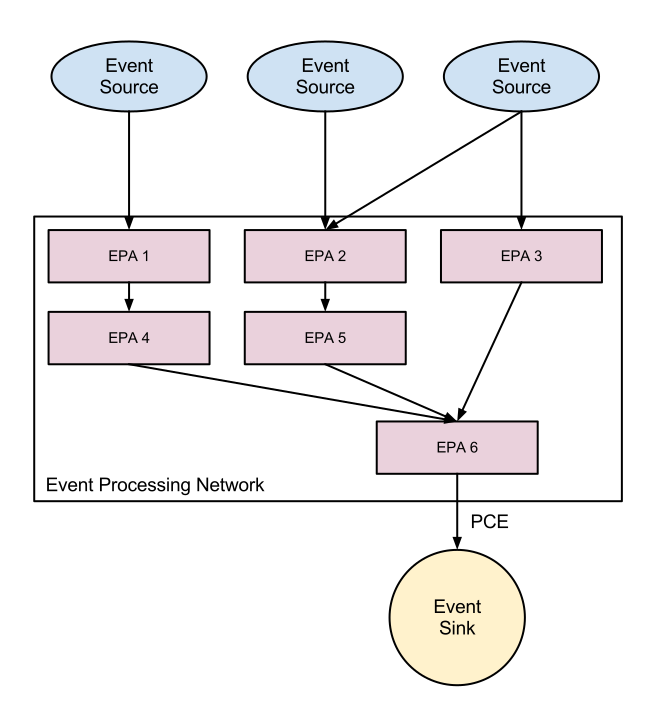
\includegraphics[scale=0.7]{images/event_processing_system.pdf}
\caption{Event Processing Network.}
\label{fig:event_processing_network}
\end{figure}

All the nodes in the network are connected via event channels (arrows in the figure). It is suggested that at this point the event channels are high-level abstractions and we do not limit the types they can handle nor the number of sources or consumers attached to them. \cite{IBM10}

A group of interconnected EPAs form an Event Processing Network (EPN). An EPN has the following properties: it can by dynamic (EPAs can be created and destroyed), it may contain feedback loops and it can be distributed across multiple physical computers. \cite{Luckham08} However, in the study case of this thesis we do not need any of those properties because the complex events we are interested in are rather simple ones.

As a result, an EPN produces a Primary Complex Event (PCE) that goes to the event sink. A PCE has the prefix primary in order to distinguish it from the complex events passed between EPAs. A PCE is the event whose future occurrences we are trying to predict in this thesis. The event sink represents all the parties who are interested in the complex event in question, including both automated machines that are triggered to perform some action and human workers who are notified when something interesting happens. \cite{Fulop12}


\section{CEP Engines and Processing Languages}
There is a wide range of Complex Event Processing Engines with different properties available on the market. First started in the Bell Labs in the mid 90's, the CEP business sector has spanned into more than 20 widely used products from all the major IT houses, such as IBM, Microsoft and Oracle. \cite{Vincent11}  

CEP engines can be divided into four subcategories based on abstraction type for event detection and action triggering. In the first category, Data Stream Query Languages, a SQL-like language is used to create relational queries against the data stream. In the second category, Production Rule Languages, queries are based on a set of condition-action pairs stored in the working memory. When a condition becomes true, the corresponding actions is fired. In the third category, Composition-Operator-Based Languages, operators are used to define complex causal queries based on simple queries, such as whether or not a certain event happens. The last category is rarer; the languages in it use logical XML formulas for automated reasoning in a Semantic Web. \cite{Bui08}

Most CEP engines have several common features that are used to handle the data stream. As all the events in CEP are somehow typed, filtering can be used to select only the ones that we are interested in. Windows, specified either with time interval or a number of events, allow us to use a subset of the stream for processing. Data aggregation, conjunctions and disjunctions can be used to create more abstract levels of events. Temporal and causal relationships between events are efficient in reasoning complex sequences and patterns of events. Of course, negation and counting methods are available for detecting the presence or absence of events. \cite{Marcelo09}

In MMEA program, and consequently in this thesis, we use an open-source, Java-based CEP engine called Esper. Esper has properties from the first three categories listed above. It uses Event Processing Language (EPL) to specify expressions for pattern matching and for detecting the presence or absence of events \cite{EsperReference}. A standard EPL query is of the form

\begin{Verbatim}[xleftmargin=1.5em]
INSERT INTO
	[stream]
SELECT
	[attributes]
FROM
	[stream]
WHERE
	[condition]
GROUP BY
	[attribute]
HAVING
	[condition]
\end{Verbatim}

The \emph{SELECT} clause is used to select which attributes we want to catch from each event that matches our filter. The optional \emph{INSERT INTO} clause puts these attributes into a new stream. The \emph{FROM} clause specifies the streams and corresponding time windows we are looking into. The \emph{WHERE} clause can filter the events, for example, by giving a threshold value for a certain event attribute. The \emph{GROUP BY} clause is used to aggregate several events of the same type into an abstraction event, for instance, by event type. The \emph{HAVING} clause is used filter the aggregated events formed by \emph{GROUP BY}. \cite{Bui08} 

In Esper, Events can be POJOs (Plain Old Java Objects), Maps (key-value-dictionaries) or XML documents. All event types have attributes that can further have sub-attributes of any type. \cite{EsperReference} In the following, I will present some examples of Java POJOs in Esper.

Say we have the following Java class
\begin{Verbatim}[xleftmargin=1.5em]
public class Sensor {
	int id;
	String name;
	Sensor[] groupSensors;  
}
\end{Verbatim}

A Sensor has an identification number, name and a list of other sensor belonging to the same group. Furthermore, say we have an event type called \emph{SensorEvent} which represents a single measurement that comes from a sensor:
\begin{Verbatim}[xleftmargin=1.5em]
public class SensorEvent {
	Sensor sensor;
	Timestamp timestamp;
	Map<String, Double> measurements;
}
\end{Verbatim}

A \emph{SensorEvent} has a reference to the sensor from which the event originated, a timestamp that captures the exact point in time when the measurement was made and a map that contains key-value pairs where the key is the variable name (e.g. temperature) and the value is the measurement value (e.g. 10.9 degrees celsius).

Now we can refer to the event attributes in an EPL query in the following way:

\begin{description}
	\item[Simple: SensorEvent.timestamp] \hfill \\
	measurement time
	\item[Nested: SensorEvent.sensor.id] \hfill \\
	sensor id
	\item[Indexed: SensorEvent.sensor.groupSensors{[0]}.name] \hfill \\
	name of the first sensor in the same group
	\item[Mapped: SensorEvent.measurements('temperature')] \hfill \\
	value of the temperature measurement
\end{description}

Next, I will present some examples of the query types we might need in the study case of this thesis. To select the name of the sensors that have the temperature exceeding 20.0 degrees can be done using the following query:

\begin{Verbatim}[xleftmargin=1.5em]
SELECT 
	sensor.name 
FROM 
	SensorEvent 
WHERE 
	measurements('temperature') > 20.0
\end{Verbatim}

To retrieve the average humidity from each sensor every 30 minutes we can use a timed window:
\begin{Verbatim}[xleftmargin=1.5em]
SELECT 
	avg(measurements('humidity')) 
FROM 
	SensorEvent.win:time_batch(30 min) 
GROUP BY 
	sensor.id
\end{Verbatim}

To define a sliding window of 30 minutes that is triggered on every new instance, we can change the \emph{win:time\_batch} to just \emph{win:time}. A time interval can be defined with \emph{timer:interval}. Combined with the patterns described below, it is useful, for example, when a certain event has to happen within 10 minutes of another event.


As an example of event pattern detection, let's assume we have a stream (called Stream) of events: $A_1 \ A_2 \ B_1$. This example was originally shown in Esper Reference \cite{EsperReference}. Now the pattern

\begin{Verbatim}[xleftmargin=1.5em]
SELECT 
	every a=A -> b=B 
FROM 
	Stream
\end{Verbatim}
matches each A followed by B ([$A_1 \ B_1$], [$A_2 \ B_1$]) but the pattern

\begin{Verbatim}[xleftmargin=1.5em]
SELECT 
	every a=A -> (b=B and not A) 
FROM
	Stream
\end{Verbatim}

matches every A followed by B but not A. In this case, the resulting event is only [$A_2 \ B_1$].


As one can see, by combining windows, relational clauses and SQL-like procedures, such as sub-queries and joins, we are able to define quite complex queries that would be hard to implement in conventional programming methods. This thesis does not focus much on the writing of effective EPL queries for detecting complex events, but rather assumes that the queries have already been defined by some domain expert. 

By default, Esper uses system's time when creating windows and handling causality. This behavior can be bypassed by turning Esper's internal clock off and constantly sending \emph{CurrentTimeEvent} objects into the engine with a selected timestamp. \cite{EsperReference} 


\section{Applications of CEP}
Complex event processing (CEP) has found applications in many fields from Business Process Monitoring (BPM) to intrusion detection in computer networks. In this chapter I present some successful examples of using CEP for high-speed data processing.

Radio frequency identification (RFID) is a technology for identifying physical objects by equipping them with a remote-readable tags that can be read using radio-frequency electromagnetic fields. Then, the lifespan of the object can be monitored more accurately than with any other method. In big industrial companies this produces a huge amount of data that has to processed and analyzed in real-time in order to get the maximum benefit from the RFID technology. CEP provides a great platform for filtering the RFID data, aggregating semantic information into the data and routing the data to customers and suppliers. \cite{Wang06}  

In the financial sector, where tremendous amounts of data are passed between banks and customers constantly, it is no surprise that the data can be transferred and processed effectively with CEP. Example use cases are detecting suspicious money transfers and credit card frauds by monitoring where the credit card has been used and how much money has been withdrawn with it. In stock market CEP can be used to follow market trends and correlations between different stocks. \cite{Adi06}

Business process management (BPM) and CEP can be integrated to provide valuable information to customer relationship management (CRM). By monitoring real-time customer interactions, such as clicks in an e-commerce or comments on a blog, business providers can create automated actions that personalize service to each customer. Event-driven actions can even indicate the customer's emotional state, which may be used for targeted advertising. \cite{Kobielus08}

In combination with predictive analytics (PA), which we will discuss more in chapter 3, CEP can be utilized to detect and locate failures in component based systems by online tracking. Chen et al. \cite{Chen06} monitored the distribution between signal and noise subspaces, and detected failures with online distribution learning algorithms. 

